\documentclass{article}
\usepackage{amsmath}
\usepackage{amssymb}
\usepackage{geometry}
\usepackage{graphicx}
\usepackage{hyperref}
\usepackage{graphicx}
\usepackage{caption}
\usepackage{subcaption}
\usepackage{amsmath}
\usepackage{float}
\usepackage{listings} 
\usepackage{color}

\title{Gaussian Process Regression From Scratch}
\author{Manthan Bagade, Anay}
\date{July 2025\thanks{Thanks to Coding Club, IITG for this assignment.}}

\begin{document}
\maketitle

\section{Introduction}
\label{sec:introduction}
\textbf{Gaussian Process Regression (GPR)} is a powerful \textbf{non-parametric Bayesian} approach that is particularly useful when dealing with problems involving continuous data, where the relationship between input variables and output is not explicitly known or can be complex. It can model certainty in predictions, making it a valuable tool for various applications, including optimization, time series forecasting, and more. \newline
We have implemented GPR from scratch using Python, which allows us to understand the underlying mechanics of the algorithm and how it can be applied to real-world problems. To keep it simple and intuitive, we have implemented only one kernel (refer \autoref{label:kernel}), the Radial Basis Function (RBF) kernel, for the time being. The code, along with some experiments and results is available on GitHub at \url{https://github.com/yourusername/GPR}.
\section{Why GPR?}
\label{sec:why_gpr}
Gaussian Process Regression (GPR) is a non-parametric, Bayesian approach to regression. It provides not just predictions, but also confidence intervals (uncertainty estimates) for those predictions. This is particularly useful in scenarios where understanding the uncertainty of predictions is crucial, such as in medical diagnosis, financial forecasting, and environmental modeling. It does not assume a functional form for the relationship between input and output, making it flexible for various types of data. GPR can also handle noisy observations effectively, providing a robust framework for regression tasks. In summary, GPR has several advantages over traditional regression methods such as :
\begin{itemize}
    \item \textbf{Non-parametric Approach:} GPR does not assume a fixed form for the underlying function, allowing it to fit to data with complex relations.
    \item \textbf{Uncertainty Quantification:} It provides not only predictions but also the confidence level of these predictions at each point.
    \item \textbf{Flexibility:} GPR can use multiple kernels, or a combination of them to model different types of the data based on the user's requirements.
    \item \textbf{Robustness to Noise:} It can effectively handle noisy observations and control the noise level, modeling real world problems.
    \item \textbf{Regularization:} GPR inherently includes a regularization mechanism through the kernel function, which helps prevent overfitting.
\end{itemize}

\section{Kernel}
\label{label:kernel}
The \textbf{Kernel} function is the most important component of GPR. It defines the similarity between points in the input space and is used to compute the covariance matrix of the Gaussian Process. The choice of kernel function can significantly affect the performance of GPR, determines the shape of the functions model is trying to learn, and the confidence it has in its predictions. Different kernels can capture different types of relationships in the data, such as periodicity, smoothness, or linearity.
\newline
There are several types of kernel functions available such as \textbf{Linear, Polynomial, Exponential, Matern, and Radial Basis Function (RBF)}. Each kernel has its own characteristics and is suitable for different types of data. Furthermore, You can combine different types of kernels to create a custom kernel that fits your specific problem by addition or multiplication of this standard kernels.
\newline 
In this implementation, we use the \textbf{Radial Basis Function (RBF)} kernel, also known as the Gaussian kernel. It is particularly popular due to its ability to model smooth functions and its infinite differentiability, making it a good choice for many regression tasks. \textbf{RBF} is defined as:
\begin{equation}
    k(x, x') = \sigma^2 \exp\left(-\frac{||x - x'||^2}{2l^2}\right)
\end{equation}
where \( \sigma^2 \) is the variance, \( l \) is the length scale, and \( ||x - x'||^2 \) is the squared Euclidean distance between the input points \( x \) and \( x' \). The parameters \( \sigma^2 \) and \( l \) control the amplitude and smoothness of the function, respectively.

\begin{figure}[H]
    \centering
    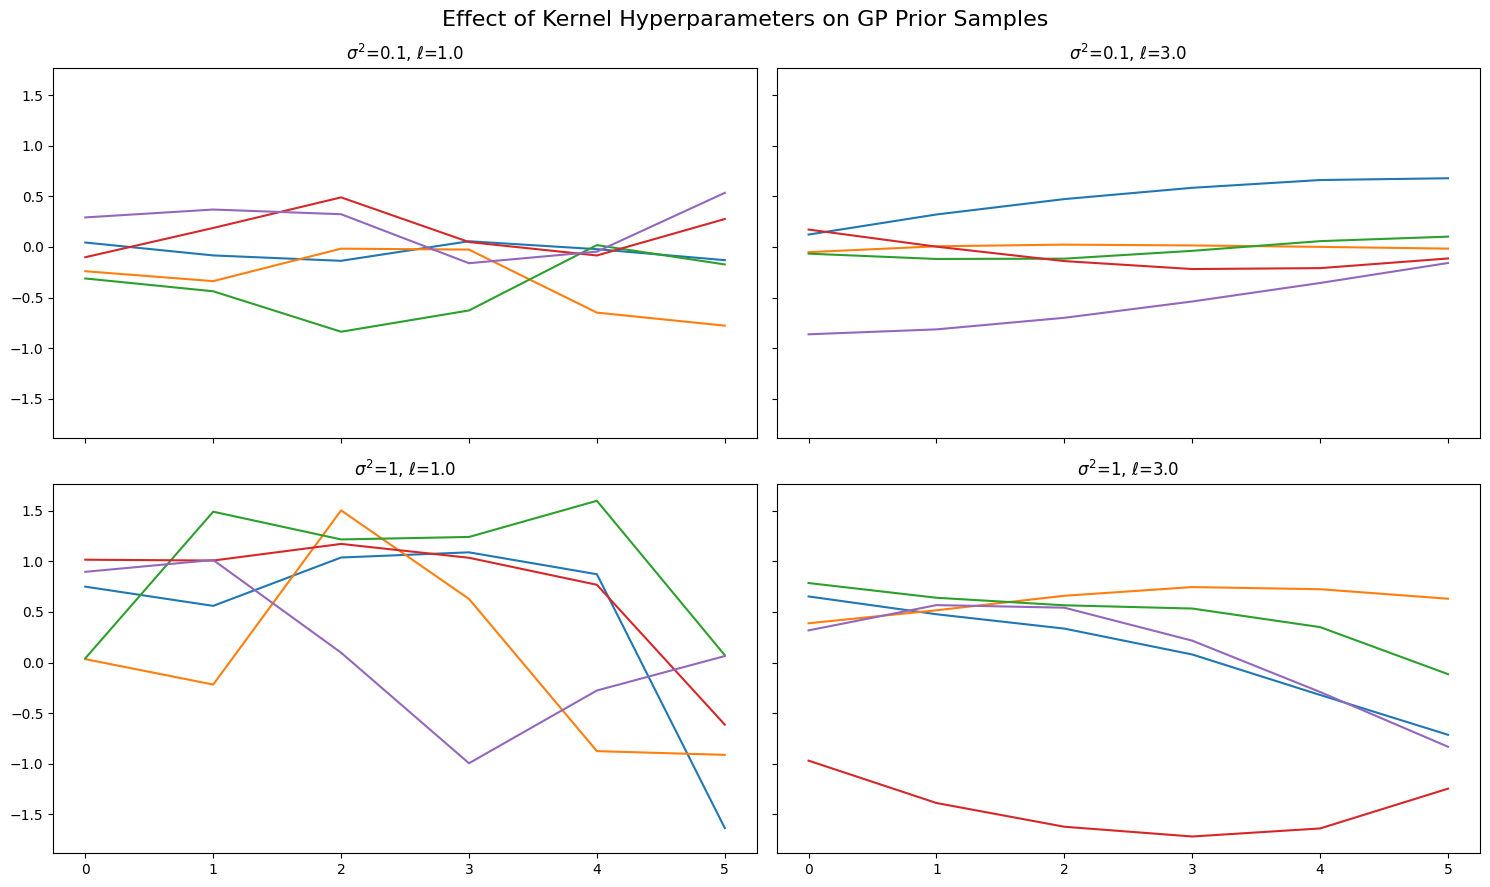
\includegraphics[width=1\textwidth]{images/kernel_hp.png}
    \caption{RBF Kernel Visualization}
    \label{fig:rbf_kernel}
\end{figure}

\section{The Algorithm}
\label{sec:algorithm}
The Gaussian Process Regression algorithm can be summarized in the following steps:
\begin{enumerate}
\item \textbf{Define the Kernel:} The user will choose a kernel function that defines the covariance between points in the input space. In our case, we use the Radial Basis Function (RBF) kernel.
\item \textbf{Compute the Covariance Matrix:} For a given set of training data points, compute the covariance matrix \( K_{11} \) using the kernel function. This matrix captures the relationships between all pairs of training points.   
\item \textbf{Add Noise:} If the observations are noisy, add a noise term to the diagonal of the covariance matrix to account for observation noise. This results in a modified covariance matrix \( K_{11} + \sigma_n^2 I \), where \( \sigma_n^2 \) is the noise variance and \( I \) is the identity matrix.
\item \textbf{Compute the Inverse:} Compute the cholesky decomposition of the covariance matrix. Using this decomposition, you can efficiently compute the inverse of the covariance matrix and using cholesky solve function you can quickly compute $K_{11}^{-1} y$.
\item \textbf{Make Predictions:} For a new input points \( X_test \), compute the covariance matrix \( K_{21} \) between the training points and the test point, and the covariance matrix \( K_{22} \) for the test point itself. The predictive mean and variance can then be computed using these quantities using the formulas. The formula for the predictive mean \( \mu \) and variance \( \sigma^2 \) is given by:
\begin{equation}
\mu = K_{21} K_{11}^{-1} y
\end{equation} 
\begin{equation}
\Sigma = K_{22} - K_{21} K_{11}^{-1} K_{12}
\end{equation}
To know more about the formulas, refer to \cite{peterroelants}.
\item \textbf{Loss Function:} The loss function is typically the negative log marginal likelihood, which can be computed using the covariance matrices and the observed outputs. This loss function can be minimized to optimize the hyperparameters of the kernel.
\begin{equation}
\text{Loss} = \frac{1}{2} y^T K_{11}^{-1} y + \log |K_{11}| + \frac{n}{2} \log(2\pi)
\end{equation}
where \( n \) is the number of training points. The first term represents the fit of the model to the data, the second term penalizes large covariance matrices, and the third term is a constant that does not depend on the parameters.
\end{enumerate}

\section{Implementation}
\label{sec:implementation}
The implementation of GPR is done in Python, utilizing libraries such as NumPy for numerical computations and Matplotlib for visualization. The code is structured to allow easy modification of the kernel function and hyperparameters. The implementation is done in two phases:
\subsection{Kernels}
In this phase, we define thekernel functions and their hyperparameters. The RBF kernel is already implemented, and you can easily add more kernels by defining their respective functions.
\lstset{
  language=Python,
  basicstyle=\ttfamily\small,
  breaklines=true,           
  breakatwhitespace=true,    
  captionpos=b,              
  showstringspaces=false,   
  keywordstyle=\color{blue},
  commentstyle=\color{green},
  stringstyle=\color{red}
}
\begin{lstlisting}
class RBFKernel:
  def __init__(self, variance = 1.0, length_scale = 1.0):
    self.variance = variance
    self.length_scale = length_scale

  def __call__(self, X1, X2):
    K = (self.variance)*(np.exp(-cdist(X1, X2, 'sqeuclidean')/(2*self.length_scale**2)))
    return K
\end{lstlisting}
\subsection{GPR Class}
In this phase, we implement the GPR class that uses the kernel to perform regression. The class includes methods for fitting the model to training data, making predictions, and computing the loss function.
\begin{lstlisting}
class GaussianProcessRegressor:
  def __init__(self, kernel, noise_variance = 1e-8) -> None:
    self.kernel = kernel
    self.noise_variance = noise_variance
    self.X_train = None
    self.y_train = None

  def fit(self, X, y) -> None:
    self.X_train = X
    self.y_train = y
    self.K11 = self.kernel(X,X) + self.noise_variance*np.eye(X.shape[0])
    self.L = cholesky(self.K11, lower=True)
    self.alpha = cho_solve((self.L, True), y)

  def predict(self, X) :
    K21 = self.kernel(X, self.X_train)
    mean = K21 @ self.alpha
    K22 = self.kernel(X, X)
    var = K22 - (K21 @ cho_solve((self.L, True), K21.T))
    diag_indices = np.diag_indices_from(var)
    var[diag_indices] = np.clip(var[diag_indices], 1e-8,np.inf)
    return mean, var
  def loss(self):
    negative_log_marginal_likelihood = self.y_train.T @ self.alpha
    penalty_term = 2*np.sum(np.log(np.diag(self.L)))
    constant_term = self.X_train.shape[0]*np.log(2*np.pi)
    return 0.5*(negative_log_marginal_likelihood+penalty_term+constant_term)
\end{lstlisting}
\section{Results}
\label{sec:results}
We have tested the GPR implementation on a synthetic dataset - sine function with some added noise, and compared our model's performace with that of sklearn. Our goal is not to model the data perfectly, but to create alike sklearn's GPR model and test it. The results show that our implementation can effectively capture the underlying function and provide uncertainty estimates for the predictions.
\begin{figure}[H]
    \centering
    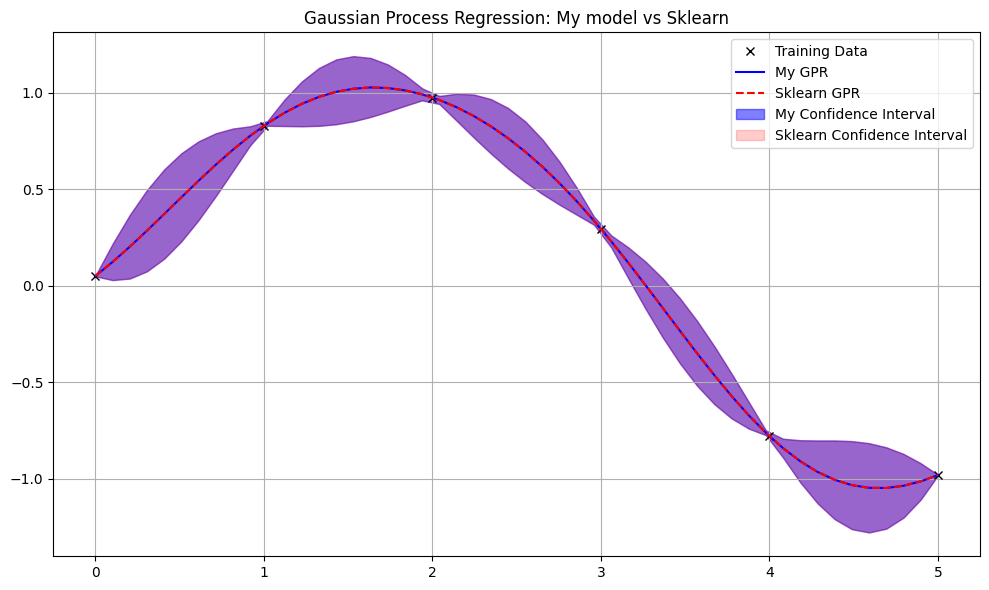
\includegraphics[width=1\textwidth]{images/sine.png}
    \caption{GPR Results on Synthetic Data}
    \label{fig:gpr_results}
\end{figure}

\begin{thebibliography}{9}
\bibitem{distill.pub}
\href{https://distill.pub/2019/visual-exploration-gaussian-process/#Multivariate}{\textit{Visual Exploration of Gaussian Processes}}, by Distill, 2019.
\bibitem{peterroelants}
\href{https://peterroelants.github.io/posts/gaussian-process-tutorial/}{\textit{Gaussian Process - From Scratch}}, by Peter Roelants.
\bibitem{scikit-learn}
\href{https://scikit-learn.org/stable/modules/gaussian_process.html}{\textit{Gaussian Processes}}, by Scikit-learn.
\bibitem{dsstackexchange}
\href{https://datascience.stackexchange.com/questions/31947/how-do-i-interpret-the-length-scale-parameter-of-the-rbf-kernel}{\textit{How do I interpret the length scale parameter of the RBF kernel?}}, on Data Science Stack Exchange.
\bibitem{gfg}
\href{https://www.geeksforgeeks.org/machine-learning/gaussian-process-regression-gpr/}{\textit{Gaussian Process Regression (GPR)}}, by GeeksforGeeks, July 24 2025.
\end{thebibliography}
\end{document}